% Created 2014-12-17 Wed 16:24
\documentclass[11pt]{template/openetcs_report}
\usepackage{fixltx2e}
\usepackage{graphicx}
\usepackage{longtable}
\usepackage{float}
\usepackage{wrapfig}
\usepackage{rotating}
\usepackage[normalem]{ulem}
\usepackage{amsmath}
\usepackage{textcomp}
\usepackage{marvosym}
\usepackage{wasysym}
\usepackage{amssymb}
\usepackage{hyperref}
\tolerance=1000
\usepackage{todonotes}
\usepackage{pdfpages}
\hypersetup{
  pdfkeywords={},
  pdfsubject={},
  linkbordercolor 	= {1 1 1},
  pdfcreator={Emacs 24.3.1 (Org mode 8.2.4)}}
%===========================
% Graphicpath
%===========================
\graphicspath{{./template/}{.}{./images/}}
%===========================
% Todo note margin
%===========================
\setlength{\marginparwidth}{7em}
%\let\oldmarginpar\marginpar
%\renewcommand\marginpar[1]{\-\oldmarginpar[\raggedleft\footnotesize #1]%
%{\raggedright\footnotesize #1}}
%===========================


\begin{document}
\frontmatter
\project{openETCS}


%assign a report number here
\reportnum{OETCS/WP7/07.3.5}

%define your workpackage here
\wp{Work-Package 7: ``Toolchain''}

%set a title here
\title{OpenETCS Roadmap}

%set a subtitle here
%\subtitle{}

%set the date of the report here


\date{\today}
\title{Traceability Architecture alternate solutions}
\subtitle{WP7 Proposition}
%define a list of authors and their affiliation here

\creatorname{Raphael Faudou}
\creatoraffil{University Bremen}
\techassessorname{}
\techassessoraffil{}

\qualityassessorname{}
\qualityassessoraffil{}

\approvalname{}
\approvalaffil{}
\author{Cecile Braunstein}
\affiliation{University Bremen}

\author{Raphaël Faudou}
\affiliation{Samares Engineering on behalf of ENSEEIHT}


% define the coverart
\coverart[width=350pt]{openETCS_EUPL}

%define the type of report
\reporttype{OpenETCS : Position Paper on traceability}


\begin{abstract}
%define an abstract here
This document presents alternate solutions to the current tool chain traceability
architecture.
\end{abstract}


\maketitle
\tableofcontents

\newpage
%=============================

% The actual document starts below this line
%=============================
%Start here
%=============================
% Document Managment
%=============================
\chapter{Document Information}

\begin{tabular}{|p{4.4cm}|p{8.7cm}|}
\hline
\multicolumn{2}{|c|}{Document information} \\
\hline
Work Package &  WP7  \\
Deliverable ID or doc. ref. & O7.3.5\\
\hline
Document title &Traceability Architecture in OpenETCS \\
Document version & 00.02 \\
Document authors (org.)  & Cécile Braunstein (Uni.Bremen) \\
\hline
\end{tabular}

\begin{tabular}{|p{4.4cm}|p{8.7cm}|}
\hline
\multicolumn{2}{|c|}{Review information} \\
\hline
Last version reviewed &  \\
\hline
Main reviewers &  \\
\hline
\end{tabular}

\begin{tabular}{|p{2.2cm}|p{4cm}|p{4cm}|p{2cm}|}
\hline
\multicolumn{4}{|c|}{Approbation} \\
\hline
  &  Name & Role & Date   \\
\hline  
Written by    &  Cécile Braunstein & WP7-T7.3 Sub-Task  & 06.02.2014 \\
&  & Leader&\\
\hline
Approved by &  &   &  \\
\hline
\end{tabular}

\begin{tabular}{|p{2.2cm}|p{2cm}|p{3cm}|p{5cm}|}
\hline
\multicolumn{4}{|c|}{Document evolution} \\
\hline
Version &  Date & Author(s) & Justification  \\
\hline  
00.00 & 17.12.2014 & C. Braunstein  &  Document creation  \\
\hline  
00.00 & 23.10.2015 & R. Faudou  &  Precisions concerning OpenETCS requirements and models and update of tool chain traceability requirements  \\


\hline  
\end{tabular}
\newpage
%==========================================
\mainmatter
%----------------------
\chapter{Introduction}
\section{Document purpose}
This document presents a proposition concerning support of openETCS project traceability activity by openETCS tool chain. This proposition is a consensus between traceability needs, project policy (open source solutions), time and efforts (focus on existing tools and features) and risks about tool maturity.

\section{Document scope}
This proposition is based on the needs and priorities about traceability, captured from different work packages (mainly WP3 and WP4) during October 2015, either from interviews or from reading of available project documents, especially:
\begin{itemize} 
\item Project Quality Assurance Plan - D1.3 - \cite{qa-plan}.
\item Definition of OpenETCS Development Process - D2.3a v02 - \cite{D2.3a}
\item OpenETCS Architecture and Design Specification - D3.5.0 - \cite{D3.5.0}  and D3.5.1 - \cite{D3.5.3}
\item Safety plan - D4.2.3 - \cite{D4.2.3}
\end{itemize}

The proposition done in this document is based on existing tools and existing tool capabilities with verified maturity. Document will explain limits of current proposition and will suggest axes to investigate in the future of project (roadmap).
But detailed evaluations of tools and features based on those investigations is not part of this document.

\section{Document organization}
Chapter 2 recalls openETCS project scope, development process, different needs and requirements to address, architecture and design specification.

Chapter 3 highlights main priorities concerning traceability and detailed expectations about traceability activities to support (including design, code, verification and validation).

Chapter 4 defines tool chain requirements concerning traceability.

Chapter 5 presents current traceability architecture defined to support tool chain requirements identified in chapter 4. This architecture is based on use of existing mature tools.

Chapter 6 summarizes limits of the current traceability architecture and suggests axes to investigate in order to improve traceability support by the OpenETCS tool chain.




\section{Investigation axes for improvements}
\subsectionAlternative{Requirement management and traceability tools}
Concerning requirement management and traceability there exist a lot of solutions. If we focus on open source solutions and especially those able to integrate into Eclipse platform, we find:
\begin{itemize}
\item Eclipse Requirement Modeling Framework (RMF). As mentioned on Eclipse web site, RMF is a framework to manage textual requirements through ReqIF standard requirement exchange format. There is a powerful GUI called "ProR" to configure, visualize and edit ReqIF requirements in RMF.
RMF/ProR is the natural choice for OpenETCS to support requirement management.

Alternatively to deal with the closed source path the requirement management may
be done by Reqtify Gateway of SCADE (also called "RM Gateway"). 

ProR can also be used to support traceability between requirements (native functionality) and between requirements and Papyrus models through a "proxy" connector.

\item PolarSys ReqCycle. It is a solution that focuses on requirement traceability. It can allow managing requirements (creation, edition, queries) with classification (scopes) and custom requirement data models but with very limited requirement editor. Strength is its ability to capture and aggregate traceability links coming from different sources (EMF models, C code, Java code, SysML models...) and to define own traceability links based on custom link types with potential attributes.

\end{itemize}

If we extend search to proprietary solutions, we find IBM DOORS and IBM DOORS Next requirement management products and Dassault Systems ReqTify product as leading solutions to support respectively requirement management and requirement traceability.

This second solution consists in using only one centralized Requirement database (as in solution 1) managed by one eclipse-based requirement management solution (ProR) and only one eclipse-based technology to support requirement traceability for all models (Papyrus and SCADE): PolarSys ReqCycle.

\begin{figure}[htb]
\centering
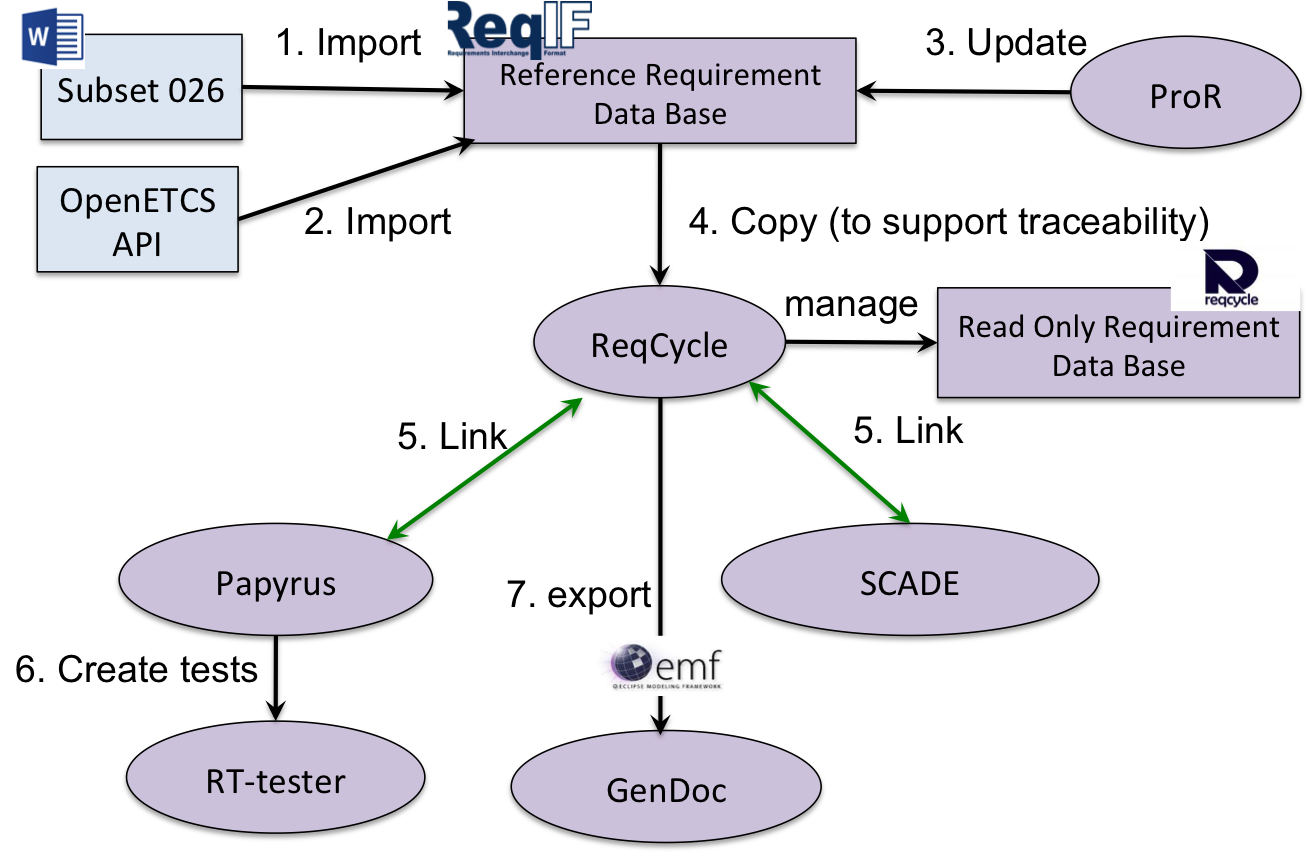
\includegraphics[width=.9\linewidth]{images/second_trace_solution-ProR-ReqCycle.png}
\caption{\label{fig:trace_second}Traceability architecture second solution}
\end{figure}

With that approach, there is still one master reference requirements data base entirely managed by ProR. Requirement database is initialized by import from the subset-026 word document, as in solution 1 (see \ref{sec-5-1}) and by import from OpenETCS API.
All new OpenETCS requirements are added in this requirement database through ProR tool.

Traceability is managed by ReqCycle tool. In order to ease visual selection of requirements in ReqCycle, there is a copy (could be a link) of reference requirements hierarchy into a ReqCycle database. Then ReqCycle manages links with Papyrus and links with SCADE. 
Finally, traceability can be exported by ReqCycle and processed by Gendoc tool to deliver documentation.

Interactions through the tool chain are detailed in figure \ref{fig:trace_second-interactions} below with focus put on traceability between requirements and functional model (traceability with SysML model, creation of tests and export of traceability are not shown here). 


\begin{figure}[tbp]
\centering
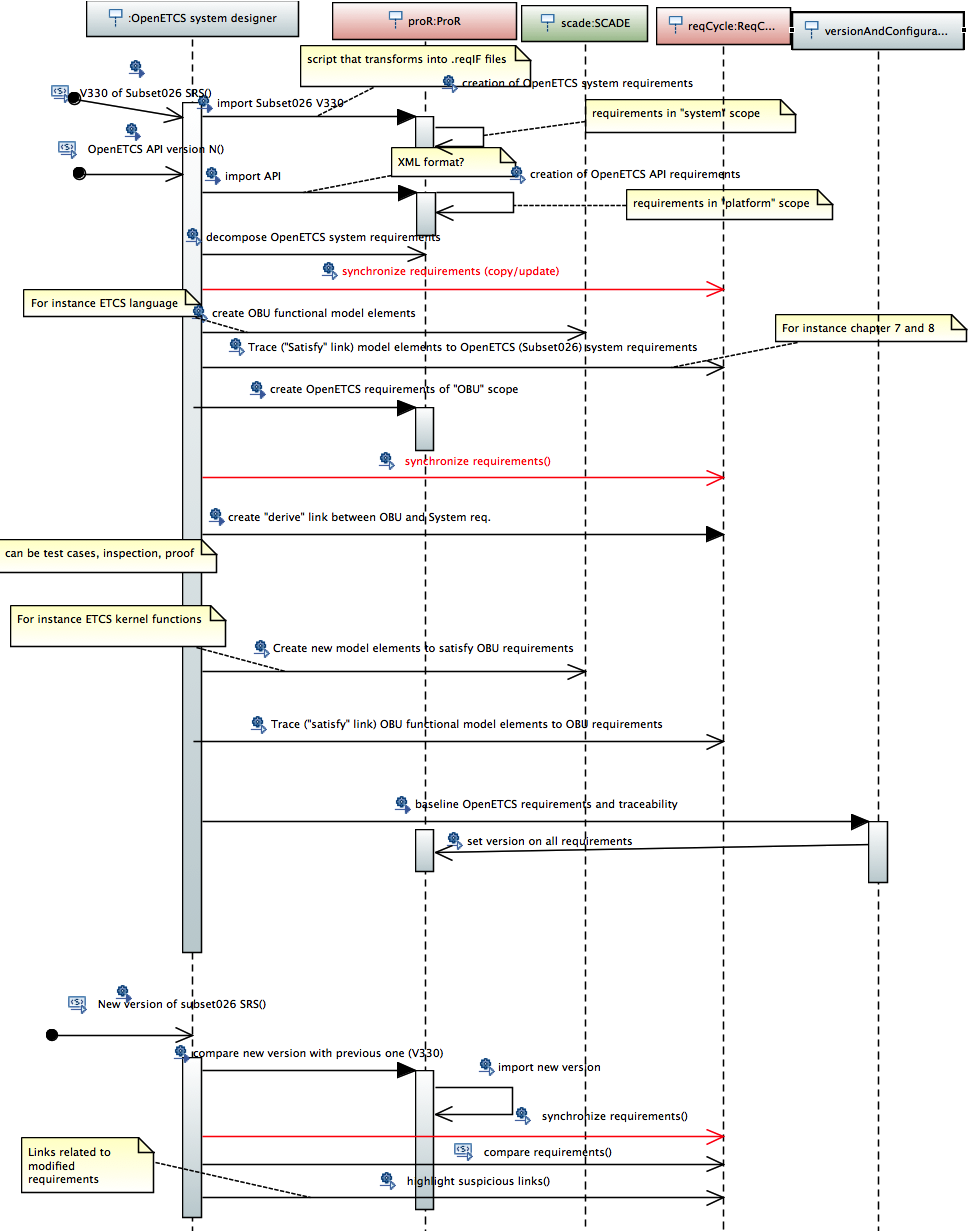
\includegraphics[width=1.0\linewidth]{images/second_trace_solution_interactions.png}
\caption{\label{fig:trace_second-interactions}second solution - interactions between tool chain components}
\end{figure}


\textbf{Note}: this solution requires synchronization from ProR to ReqCycle each time requirements change in the reference.
 
Most complex commands are detailed in next paragraphs.

\subsection{Subset-026 import}
\label{sec-6-1}
The subset-026 import can be realized by two means:
\begin{itemize}
\item Either by direct import from the subset-026 word document (ReqCycle Document import connector)
\item Or by a two steps process with transformation from word document to .ReqIF files (1.B1 path in the figure) and then import of those .ReqIF files into ReqCycle requirement database (1.B2 path).
	\begin{itemize}

	\item 1.A1 transformation can be realized with same script than the one described in first traceability solution - see \ref{sec-5-1}

	\item 1.A2 transformation (import) can be done by ReqCycle ReqIF import connector.
	\end{itemize}
\end{itemize}

\subsection{Creation of additional OpenETCS requirements}
\label{sec-6-2}
ProR can create new requirements by decomposition or by derivation of existing requirements.
In case of derivation, engineering level (scope) changes (for instance from System to OBU or to OBU Kernel).

Regularly, when there have been new requirements created, there must by a synchronization from ReqIF reference requirement database to ReqCycle internal database so that ReqCycle can manage traceability to those requirements. This synchronization is done by a ReqCycle "import or update" command from .reqIF files: first time it is an import (creation of requirements) and next times this is an update of existing requirements with ability to highlights associated traceability links (that have to be checked).

\textbf{Note}: in the future, we could have a link (reference) between ProR requirement database (ReqIF format) and ReqCycle database, rather than a copy. 

We could also have traceability driven by ReqCycle but selection of requirement done in ProR tool.

\subsection{Creation of links between SysML model elements and requirements}
\label{sec-6-3}
ReqCycle provides a view that allows creating a link between two selected objects (traceability Creator). See figure \ref{fig:trace_second-TraceabilityCreator}.

Concerning selection of requirements, ReqCycle provides a view (Requirement View) from which it is possible to select one source object. Once selection is done, it can be propagated in traceability creator view (source area).

Concerning selection of SysML model elements, Papyrus provides a view with model elements (Model explorer) from which it is possible to select a destination object. Once selection is done, it can be propagated to the traceability creator view (destination area).

When both source and destination objects are selected, ReqCycle provides a command (button) to create links between selected objects if a link type definition is compliant with such source and destination (Refinement in the illustration on figure \ref{fig:trace_second-TraceabilityCreator} below).

\begin{figure}[htbp]
\centering
\includegraphics[width=1.0\linewidth]{images/second_trace_solution_TraceabilityCreator.png}
\caption{\label{fig:trace_second-TraceabilityCreator}ReqCycle - traceability creator}
\end{figure}

\subsection{Creation of links between SCADE model and requirements}
\label{sec-6-4}
There are two approaches that can be used: 
\begin{enumerate}
\item use same approach than for creation of trace links between SysML model elements and OpenETCS requirements (see \ref{sec-6-3}).

\textbf{Note}: there is some investigation to check that it is (easily) feasible to propagate selection of a SCADE model element in ReqCycle traceability creator view (source or destination area).

\item use SCADE comment area available for any model element, fill it with traceability link data and let ReqCycle capture those traceability links by analysing SCADE model file (dedicated SCADE traceability analysis engine to implement). 

In order to avoid mistakes on editing link annotation in comment area in SCADE, idea is to generate requirement traceability link annotation from ReqCycle command ("Generate requirement traceability annotation for external element") and copy it into the clipboard. 

Then, in SCADE, system designer has just to "paste" string (from clipboard) in the concerned model element comment area and let ReqCycle analyse traceability: ReqCycle will parse SCADE model file, will capture all comments with associated model elements and will build the traceability links from requirement ID, trace link type and SCADE model element.


Figure \ref{fig:ReqCycle_PrepareTraceLinkAnnotation} illustrates such command.

\end{enumerate} 

\begin{figure}[tbp]
\centering
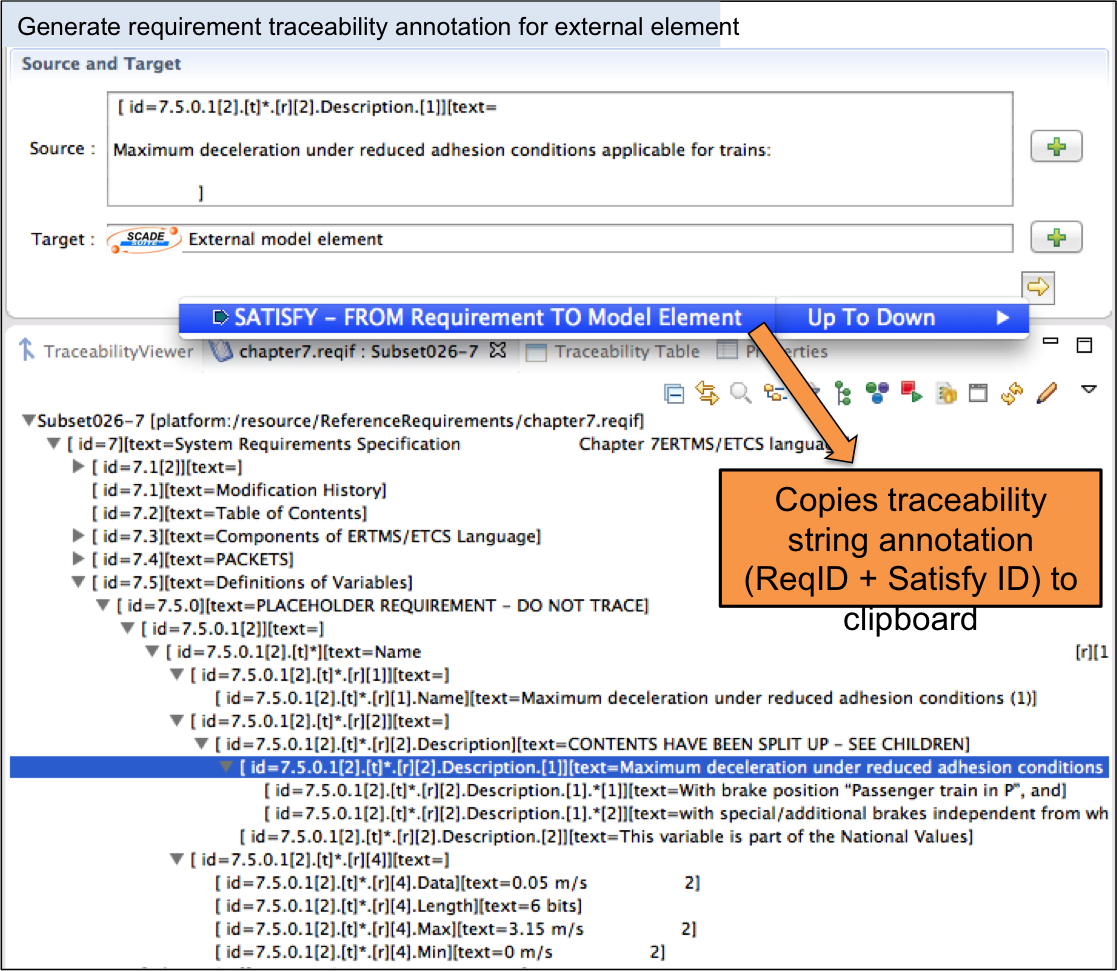
\includegraphics[width=0.9\linewidth]{images/ReqCycle_PrepareTraceLinkAnnotationForExternalElement.png}
\caption{\label{fig:ReqCycle_PrepareTraceLinkAnnotation}ReqCycle - generate traceability annotation for external model element (SCADE for instance)}
\end{figure}


\section{Aggregation of traceability links and export}
\label{sec-6-5}
It is done by ReqCycle that has all information (copy of the requirement database and associated traceability between requirements + all traceability links with models).
It is exported into EMF format that can be processed by Gendoc to render expected documentation including traceability.

\subsection{Third alternative traceability solution: ReqCycle}
\label{sec-7}
This third solution consists in using only one centralized Requirement database (as in previous solutions) managed by one eclipse-based solution (ReqCycle) also used to support requirement traceability for all models (Papyrus and SCADE).

\begin{figure}[htb]
\centering
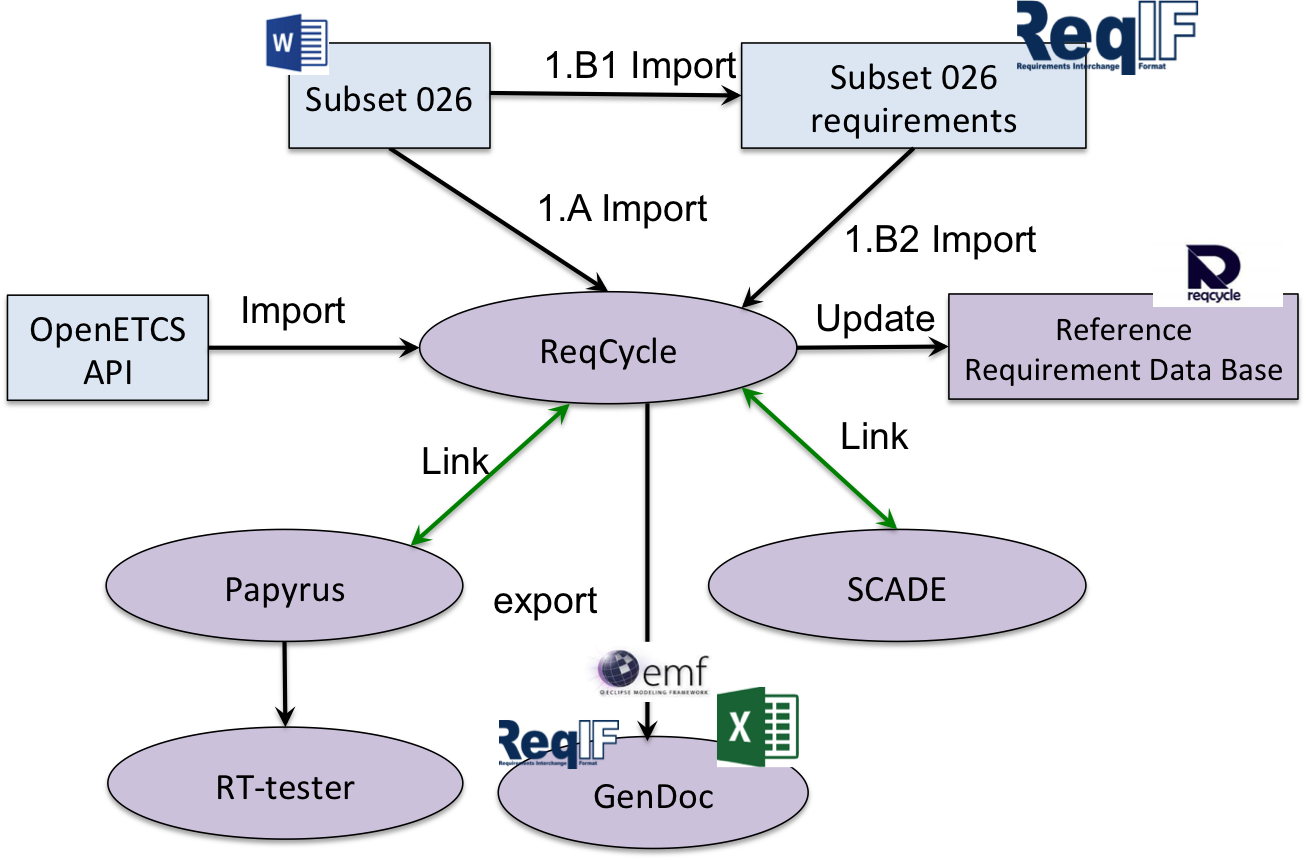
\includegraphics[width=.9\linewidth]{images/Third-Solution-ReqCycle.png}
\caption{\label{fig:trace_third}Traceability architecture third solution with ReqCycle only}
\end{figure}

With that approach, there is still one master reference requirements data base entirely managed by ReqCycle. Requirement database is initialized by import from the subset-026 word document through two possible means (see next section) and by import from OpenETCS API.
All new OpenETCS requirements are added in this requirement database through ReqCycle tool.

Traceability is managed by ReqCycle tool. In order to ease visual selection of requirements in ReqCycle, there is a copy (could be a link) of reference requirements hierarchy into a ReqCycle database. Then ReqCycle manages links with Papyrus and links with SCADE. 
Finally, traceability can be exported by ReqCycle and processed by Gendoc tool to deliver documentation.

Most complex commands are detailed in next paragraphs.


\subsection{Subset-026 import}
\label{sec-7-1}
The subset-026 import can be realized by two means:
\begin{itemize}
\item either by direct import from the subset-026 word document (ReqCycle Document import connector)
\item else by a two steps process with transformation from word document to .ReqIF files (1.B1 path in the figure) and then import of those .ReqIF files into ReqCycle requirement database (1.B2 path).
	\begin{itemize}

	\item 1.A1 transformation can be realized with same script than the one described in first traceability solution - see \ref{sec-5-1}

	\item 1.A2 transformation (import) can be done by ReqCycle ReqIF import connector.
	\end{itemize}
\end{itemize}

\section{Creation of additional OpenETCS requirements}
\label{sec-7-2}
ReqCycle provides a "local" connector to create new requirements and those requirements can be linked to existing other requirements through different kinds of links (derivation, refinement, decomposition). Those link types have to be defined first in ReqCycle configuration.

To complete

\section{Creation of links between SysML model elements and requirements}
\label{sec-7-3}
Same solution than in second solution. see \ref{sec-6-3}

\section{Creation of links between SCADE model and requirements}
\label{sec-6-4}
Same solution than in second solution. see \ref{sec-6-4}

\section{Aggregation of traceability links and export}
\label{sec-6-5}
Same solution than in second solution. see \ref{sec-6-5}



\chapter{Tool evaluations}
Will be done in a separate document.
\subsection{{\bfseries\sffamily TODO} ReqCycle  Evaluation}
\label{sec-4-5}
\subsection{{\bfseries\sffamily TODO} Reqtify Evaluation}
\label{sec-4-6}



%% Bibliography
% \nocite{*}
\bibliographystyle{unsrt}
\bibliography{oetc_WP7_Traceability}



%Examples are below


%\lipsum[11]

%\nocite{*}

%\bibliographystyle{unsrt}
%\bibliography{Lbrr}



% \begin{thebibliography}{9}

% \bibitem{lamport94}
%   Leslie Lamport,
%   \emph{\LaTeX: A Document Preparation System}.
%   Addison Wesley, Massachusetts,
%   2nd Edition,
%   1994.

% \end{thebibliography}

%===================================================
%Do NOT change anything below this line
\end{document}

%%  LocalWords:  traceability OpenETCS
